\chapter{ワークC データ取得・分析}

\section{はじめに}
現代の産業機器や民生用測定機器（ヘルスケア機器やスマート測定器など）は，物理量を電気信号へと変換する「測定機能」と，得られた情報を視覚的に伝達する「表示機能」を兼ね備えている．
さらに，近年ではIoT（Internet of Things）の急速な普及に伴い，長期間にわたるデータの蓄積や高度な統計分析を可能にするため，外部のコンピュータやクラウドシステムと連携する「通信機能」を統合したシステムが不可欠となっている．
例えばスマート体重計においては，単独で体重や体組成の測定と内蔵ディスプレイへの即時表示を行う一方，無線通信を介してスマートフォン等の上位計算機へデータを定期転送し，時系列分析や健康管理アプリケーションを担わせる構成が一般的である．

本実習（ワークC）の目的は，マイコン（Arduino UNO R4 WiFi）に標準搭載された表示デバイスおよび無線通信モジュールを活用し，センサデータの取得，可視化表示，ネットワーク配信，ならびに時系列データの信号処理に至る一連のデータ処理技術を総合的に習得することである．
本ワークは以下の3段階の課題に沿って実施した：
\begin{enumerate}
    \item \textbf{ワークC-1（LEDマトリクスを用いたデータの表示と距離測定）}：Arduino UNO R4 WiFiに内蔵された8×12赤色LEDマトリクスを用い，多次元配列の操作によって測定電圧値を小数第2位まで視覚表示するプログラムを開発した．さらに，反射型フォトリフレクタ（LBR-127HLD）を用いたセンサ回路を構築し，センサ受発光面と遮蔽物との間の距離を段階的に変化させた際の出力電圧特性を測定・グラフ化した．
    \item \textbf{ワークC-2（ネットワークを介したデータの取得とWebサーバ構築）}：Arduino UNO R4 WiFiに搭載されたESP32-S3モジュールを用いて独自のWi-Fiアクセスポイントを起動し，クライアントからの要求に応じて測定データをJSON（JavaScript Object Notation）形式で配信する組み込みWebサーバを構築した．そして，硫化カドミウム（CdS）光導電セルを用いた照度センサ回路を接続し，遮蔽物（手）の接近・離脱に伴う電圧の時間変化を，Pythonを用いたクライアントPC上のプログラムにより非同期通信で自動取得してCSV形式で記録した．
    \item \textbf{ワークC-3（時系列データの平滑化処理）}：ワークC-2で取得した照度変化の時系列電圧データに対し，計測ノイズの低減と信号トレンドの抽出を目的として，移動平均（Moving Average: MA）および指数移動平均（Exponential Moving Average: EMA）の2種類の平滑化アルゴリズムを実装・適用した．平滑化前後の波形比較を通じて，各手法におけるノイズ抑制性能と応答遅延のトレードオフを定量的に評価・考察した．
\end{enumerate}


%-----------------------------------------------------------------------------------
\section{方法及び手順}

\subsection{ワークC-1：LEDマトリクスの活用と距離測定回路}

\subsubsection{LEDマトリクスによる数値表示の設計}
Arduino UNO R4 WiFiには，基板表面に8行12列（計96個）の赤色LEDマトリクスが標準搭載されている．
表示内容は，8行12列の2値状態を保持する\texttt{byte}型2次元配列\texttt{frame[8][12]}（0：消灯，1：点灯）によって管理され，Arduino標準の\texttt{Arduino\_LED\_Matrix}ライブラリに属する\texttt{matrix.renderBitmap(frame, 8, 12)}関数を呼び出すことでLEDマトリクス上に描画される．

本ワークでは，A0ピンから取得したアナログ入力電圧（0.00〜5.00\,V）を小数第2位までの3桁の数値として表示するため，縦5ドット×横3ドットの数字フォントパターン（0〜9）を格納した2次元配列\texttt{digits[5][30]}を定義した．
3桁の数字および小数点の配置座標は，図\ref{fig:matrix_layout}に示す通りに設計した：
\begin{itemize}
    \item \textbf{百の位（整数部）}：開始座標を2行目1列目（\texttt{s\_r = 2, s\_c = 1}）とし，1〜3列目，2〜6行目に描画した．
    \item \textbf{小数点}：整数部と小数第1位の区切りを明確にするため，7行目4列目のLEDを常時点灯（\texttt{frame[7][4] = 1}）させた．
    \item \textbf{十の位（小数第1位）}：開始座標を2行目5列目（\texttt{s\_r = 2, s\_c = 5}）とし，5〜7列目，2〜6行目に描画した．
    \item \textbf{一の位（小数第2位）}：開始座標を2行目9列目（\texttt{s\_r = 2, s\_c = 9}）とし，9〜11列目，2〜6行目に描画した．
\end{itemize}

\begin{figure}[htbp]
  \centering
  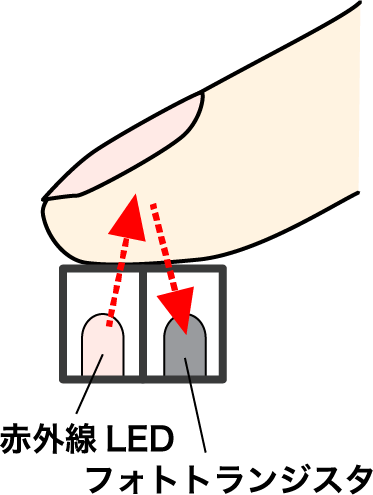
\includegraphics[width=0.6\textwidth,clip]{fig_work_C/prm.png}
  \caption{フォトリフレクタの受発光原理とLEDマトリクス表示の概念}
  \label{fig:matrix_layout}
\end{figure}

指定された数字 $d \in \{0, \dots, 9\}$ を指定座標 $(s\_r, s\_c)$ に描画する関数\texttt{displayDigitC1}では，2重の\texttt{for}ループを用いて\texttt{digits}配列から\texttt{frame}配列への値のコピーを行った：
\begin{equation}
    \texttt{frame}[s\_r + r][s\_c + c] = \texttt{digits}[r][d \times 3 + c] \quad (r \in [0, 4], c \in [0, 2])
\end{equation}
Arduino UNO R4 WiFiのA/D変換の分解能は初期設定で10ビットであり\cite{arduino_adc_resolution}，A0ピンから\texttt{analogRead(A0)}により読み取った10ビットデジタル値（0〜1023）を電圧値 $V$ に変換する計算式は，
\begin{equation}
    V = \frac{\texttt{analogValue}}{1023.0} \times 5.0\,\mathrm{[V]}
    \label{eq:adc_to_voltage}
\end{equation}
とした．この電圧値を100倍して整数化した値に対し，剰余演算および除算を用いて各桁の数値を抽出し，100\,msごとに画面を更新する構成とした．

\subsubsection{フォトリフレクタを用いた距離測定回路の構成}
距離測定部には，赤外発光ダイオードとフォトトランジスタを一体化した反射型フォトリフレクタ（LBR-127HLD\cite{LBR-127HLD}）を採用した．
回路構成を図\ref{fig:c1_circuit}に，測定時の配置の様子を図\ref{fig:c1_experiment}に示す．
赤外LEDのアノード側には電流制限抵抗 $R_D = 330\,\Omega$ を直列接続して電源電圧5\,Vを印加し，カソード側をGNDに接地した．
フォトトランジスタのコレクタ端子には負荷抵抗 $R_L = 3.3\,\mathrm{k}\Omega$ を接続して5\,Vラインにプルアップし，エミッタ端子をGNDに接地した．コレクタと抵抗 $R_L$ の接続点からセンサ出力電圧 $V_{\mathrm{out}}$ を引き出し，ArduinoのA0ピンに入力した．

\begin{figure}[htbp]
  \centering
  \begin{minipage}[b]{0.48\textwidth}
    \centering
    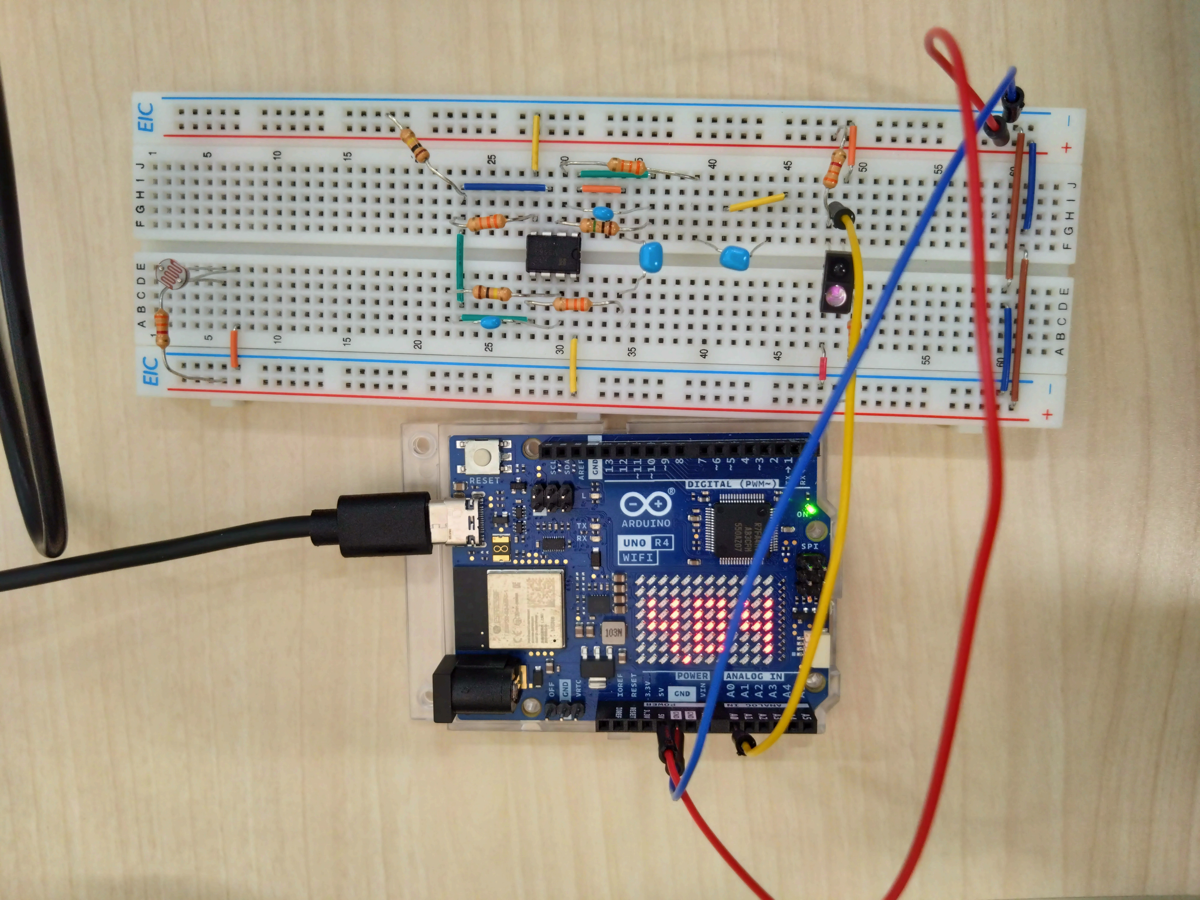
\includegraphics[width=\textwidth,clip]{fig_work_C/c1_circuit.png}
    \caption{フォトリフレクタを用いた距離測定回路}
    \label{fig:c1_circuit}
  \end{minipage}
  \hfill
  \begin{minipage}[b]{0.48\textwidth}
    \centering
    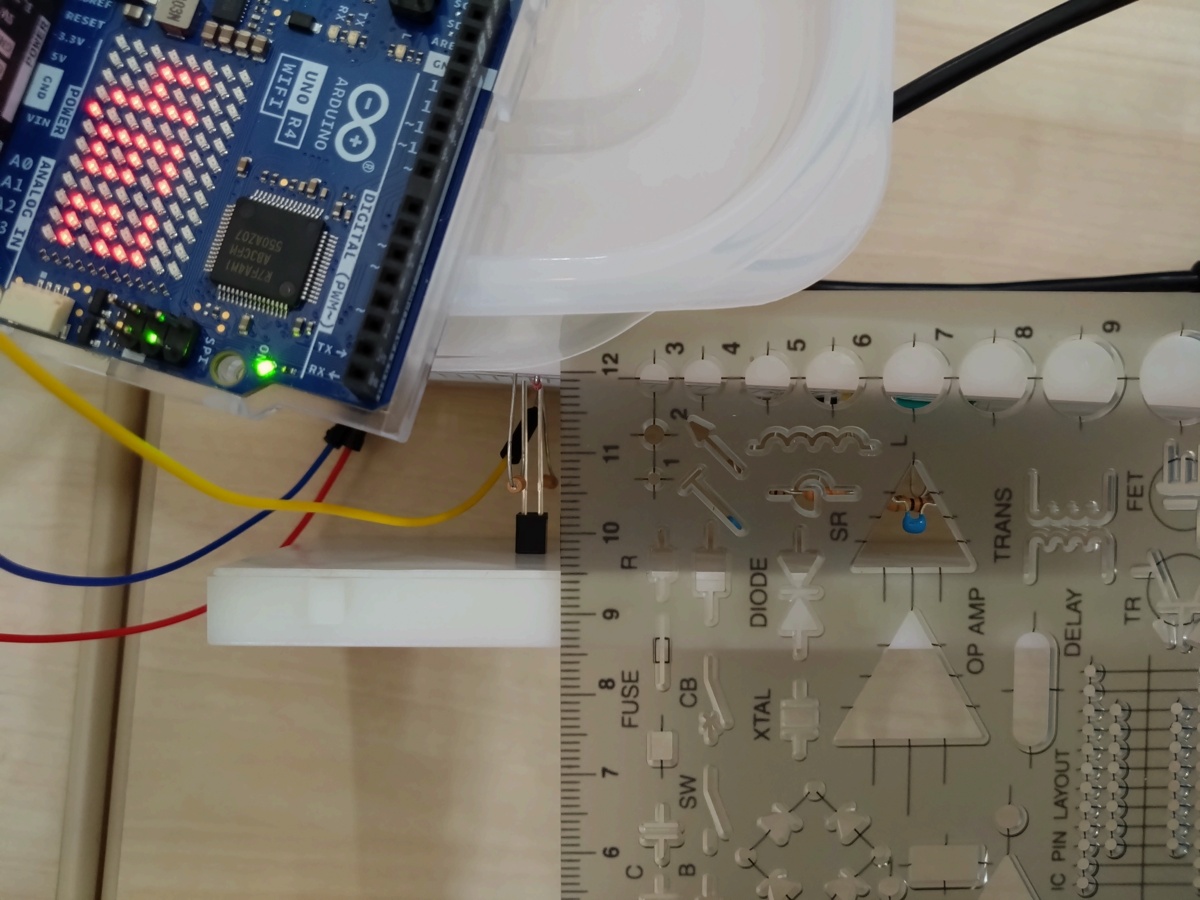
\includegraphics[width=\textwidth,clip]{fig_work_C/c1_experiment.png}
    \caption{フォトリフレクタを用いた距離測定の様子}
    \label{fig:c1_experiment}
  \end{minipage}
\end{figure}

\subsubsection{距離測定実験の手順}
実験手順は以下の通りである：
\begin{enumerate}
    \item ブレッドボード上にフォトリフレクタ回路を配線し，Arduinoの5\,V，GND，A0ピンに接続した．
    \item センサ受発光面の正面に垂直な遮蔽物（白色平板）を対向配置した．
    \item センサ受発光面と遮蔽物間の距離 $d$ を，目盛り付き定規を用いて $0.5\,\mathrm{cm}$（$5\,\mathrm{mm}$）から $5.0\,\mathrm{cm}$（$50\,\mathrm{mm}$）まで $0.5\,\mathrm{cm}$ 間隔で精密に設定した．
    \item 各距離においてLEDマトリクスに表示された電圧値，およびシリアルモニタで得られた安定電圧値を記録した．
    \item 得られた測定データをPythonスクリプト（\texttt{work\_C.py}）およびJupyter Notebook（\texttt{work\_C.ipynb}）に入力し，距離--電圧特性曲線を描画して画像（\texttt{result\_C1.png}）として保存した．
\end{enumerate}


\subsection{ワークC-2：Webサーバ構築とネットワーク経由データ取得}

\subsubsection{組み込みWebサーバの構築と通信仕様}
Arduino UNO R4 WiFiに搭載されたESP32-S3無線モジュールを利用し，外部ルータを介さずにPCと直接1対1で通信可能なSoftAP（Software Access Point）モードを設定した．
アクセスポイントのSSIDは，学籍番号（26G1012）の下3桁に基づいて \texttt{"ZZAP012"}，パスワードは空文字列（オープンネットワーク）に設定した．
IPアドレス体系として，Cクラスプライベートアドレス \texttt{192.168.12.2} を静的に割り当てた．

本ワークでは，クライアントサーバ方式によりデータを取得した\cite{rfc9110}．
Arduino上で動作するWebサーバ（\texttt{WiFiServer server(80)}）は，TCPポート80にてHTTPリクエストを監視する．
クライアント（PC）からHTTP GETリクエストを受信すると，HTTP/1.1標準に準拠したレスポンスヘッダ，および測定データを名前と値の組で表現するJSON形式のメッセージボディ\cite{rfc8259}を生成してクライアントへ返信する：
\begin{itemize}
    \item ステータスライン：\texttt{HTTP/1.1 200 OK}
    \item ヘッダ行：\texttt{Content-Type: application/json}，\texttt{Content-Length: [長さ]}，\\
          \texttt{Connection: close}
    \item メッセージボディ：\verb|{"value": X.XX}|（ここで \texttt{X.XX} はA0ピンで測定された電圧値の実数値）
\end{itemize}
データ送信完了後，\texttt{client.flush()} によりソケットバッファの送出完了を確認した上で \texttt{client.stop()} を実行し，接続を正常切断する処理とした．

\subsubsection{CdS光導電セルを用いた照度センサ回路}
ワークC-2では，環境光および遮蔽による照度変化を検出するため，光電導素子であるCdSセル\cite{川口慎一朗1966cds, 石川太郎1974照明制御システムへの半導体応用, advanced_photonix_pdv_p5002}を用いた．
センサ回路の外観を図\ref{fig:c2_circuit}に，センサ上方に手をかざして電圧を測定する様子を図\ref{fig:c2_experiment}に示す．
CdSセルは，光の照射強度（ルクス）に応じて素子抵抗値 $R_{\mathrm{CdS}}$ が大きく低下する負の光導電特性を有する．

\begin{figure}[htbp]
  \centering
  \begin{minipage}[b]{0.48\textwidth}
    \centering
    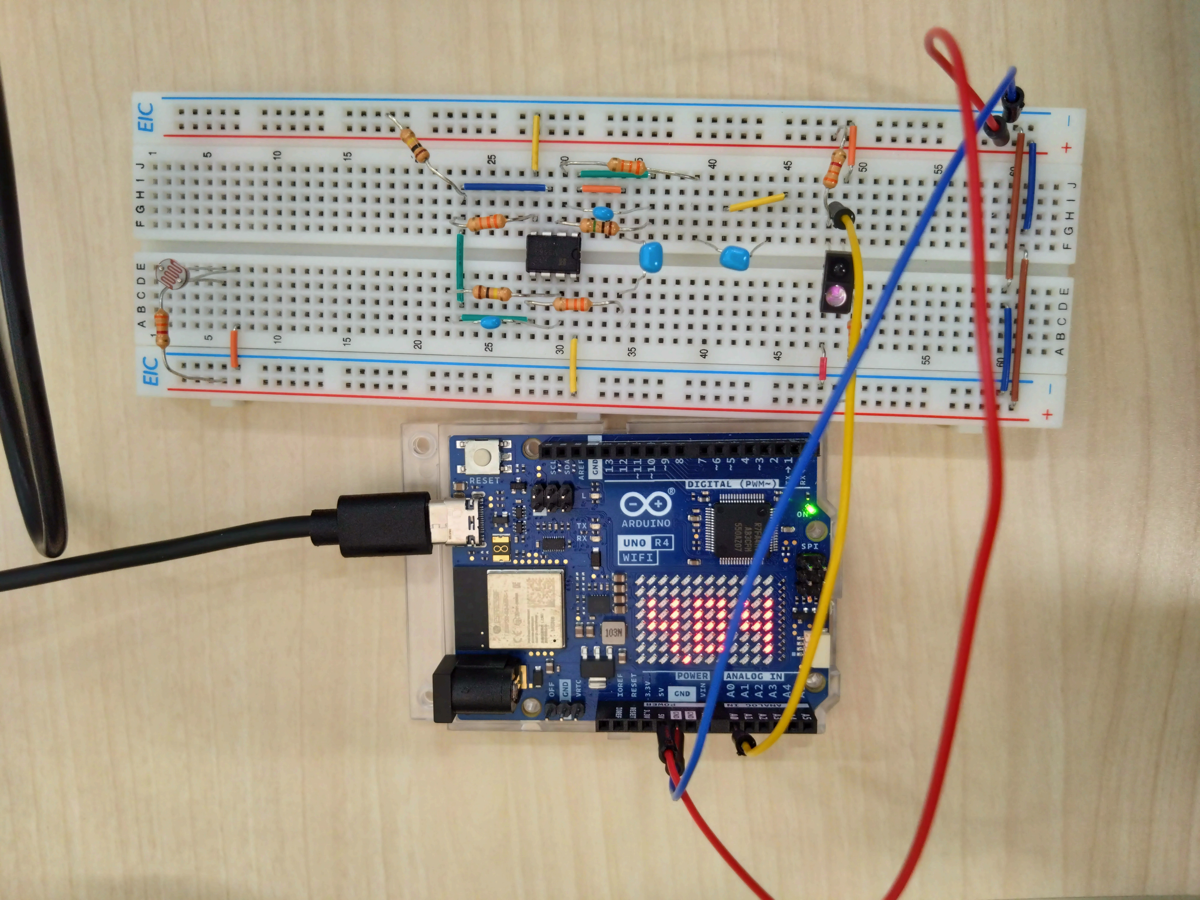
\includegraphics[width=\textwidth,clip]{fig_work_C/c2_circuit.png}
    \caption{CdSセルを用いた照度変化測定回路}
    \label{fig:c2_circuit}
  \end{minipage}
  \hfill
  \begin{minipage}[b]{0.48\textwidth}
    \centering
    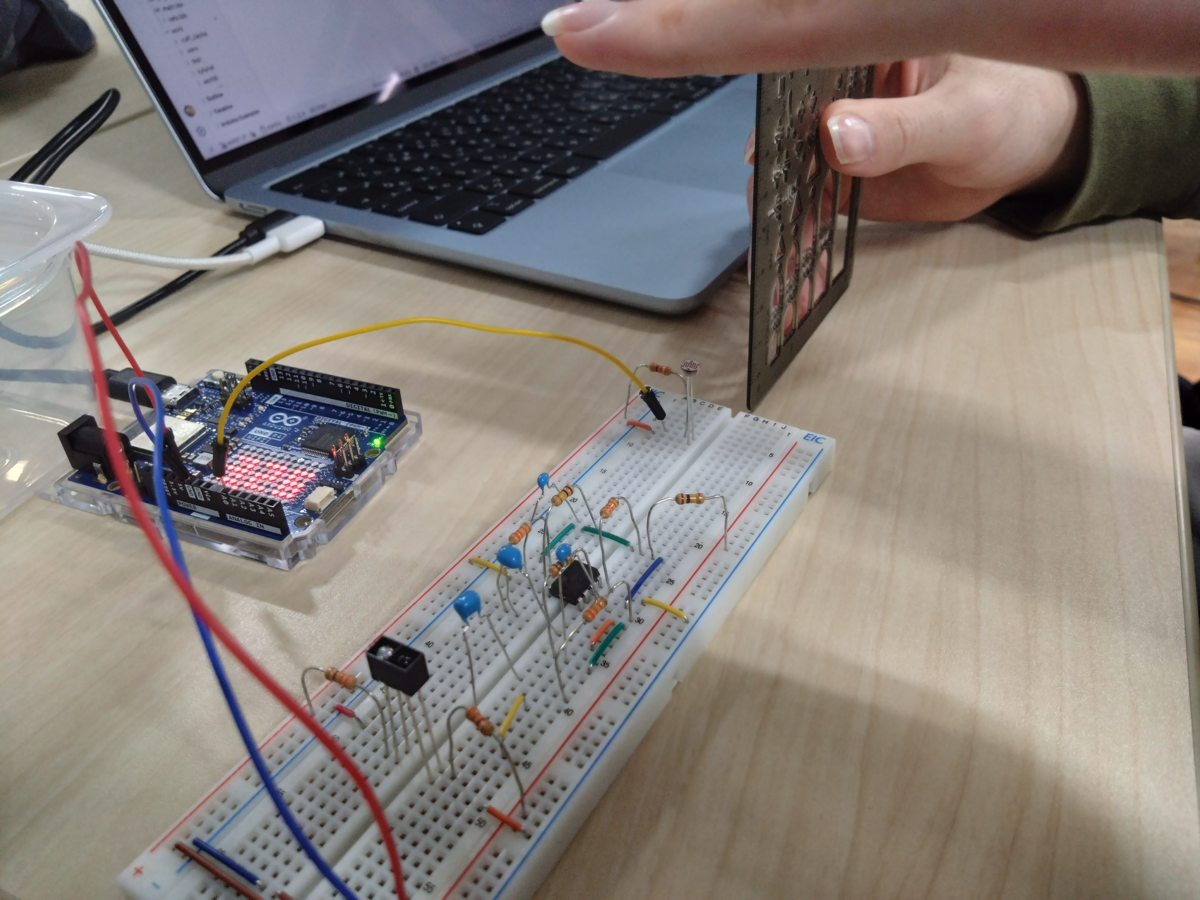
\includegraphics[width=\textwidth,clip]{fig_work_C/c2_experiment.png}
    \caption{CdSセルの上方に手をかざして電圧を測定する様子}
    \label{fig:c2_experiment}
  \end{minipage}
\end{figure}

回路構成は，電源電圧 $V_{CC} = 5\,\mathrm{V}$ とGNDの間にCdSセルと固定抵抗 $R_F = 3.3\,\mathrm{k}\Omega$ を直列に接続した分圧回路とした．
固定抵抗 $R_F$ をGND側に配置し，CdSセルと $R_F$ の接続点電位をA0ピンに接続した．
この構成における出力電圧 $V_{\mathrm{out}}$ は，
\begin{equation}
    V_{\mathrm{out}} = V_{CC} \times \frac{R_F}{R_{\mathrm{CdS}} + R_F}
    \label{eq:cds_divider}
\end{equation}
により決定される．手がセンサを覆って照度が低下すると $R_{\mathrm{CdS}}$ が増大するため，出力電圧 $V_{\mathrm{out}}$ は低下する（またはCdSの配置位置をGND側とした場合は上昇する）．
本実習では，遮蔽物（手）の接近に伴いA0電圧が単調増加するように，5\,V側に固定抵抗 $R_F = 3.3\,\mathrm{k}\Omega$，GND側にCdSセルを接続し，分圧点電位
\begin{equation}
    V_{\mathrm{out}} = V_{CC} \times \frac{R_{\mathrm{CdS}}}{R_F + R_{\mathrm{CdS}}}
    \label{eq:cds_divider_actual}
\end{equation}
をA0ピンに入力する回路を採用した．

\subsubsection{時系列データ取得手順}
PCをArduinoのアクセスポイント \texttt{ZZAP012} にWi-Fi接続した状態で，Pythonプログラム（\texttt{requests}ライブラリおよび別スレッドワーカーを用いた非同期ポーリング）を実行した．
サンプリング周期は $1.0\,\mathrm{s}$，総計測時間は $100\,\mathrm{s}$（計101サンプル）とし，以下の5段階（各20秒間）の手順により意図的な照度変化を与えた：
\begin{enumerate}
    \item \textbf{フェーズ1（0〜20\,s）}：CdSセルの受光面を天井照明に向け，センサ上部に遮蔽物が何もない開放状態で定常電圧を測定した．
    \item \textbf{フェーズ2（21〜40\,s）}：CdSセルの受光面上部約 $9\,\mathrm{cm}$ の位置に手のひらを水平にかざし，弱遮蔽時の電圧を測定した．
    \item \textbf{フェーズ3（41〜60\,s）}：CdSセルの受光面上部約 $6\,\mathrm{cm}$ の位置まで手を下降させ，中遮蔽時の電圧を測定した．
    \item \textbf{フェーズ4（61〜80\,s）}：CdSセルの受光面上部約 $3\,\mathrm{cm}$ の位置まで手を接近させ，強遮蔽時の電圧を測定した．
    \item \textbf{フェーズ5（81〜100\,s）}：手を完全に離し，再びセンサ上部を開放した状態で基線電圧への復帰挙動を測定した．
\end{enumerate}
取得した時系列データは \texttt{result\_C2.csv} に保存し，時間--電圧波形グラフ（\texttt{result\_C2.png}）を生成した．


\subsection{ワークC-3：時系列データの平滑化処理アルゴリズム}

実測されたセンサデータには，素子の熱雑音，商用電源起因のリップル，および手の微小な震え（体動）に伴うランダムノイズが重畳する．
本ワークでは，ノイズを除去して真の物理的変位傾向を抽出するため，2種類の代表的なデジタルフィルタを実装した．

\subsubsection{単純移動平均（Simple Moving Average: MA）}
移動平均法は，過去 $M$ サンプルの観測値の相加平均を順次算出する有限インパルス応答（FIR）フィルタである\cite{smith1997scientist}．
離散時刻 $n$ における入力データを $x[n]$，ウインドウサイズを $M = 5$ とすると，平滑化出力 $y_{\mathrm{MA}}[n]$ は，
\begin{equation}
    y_{\mathrm{MA}}[n] = \frac{1}{M} \sum_{k=0}^{M-1} x[n-k] = \frac{x[n] + x[n-1] + x[n-2] + x[n-3] + x[n-4]}{5}
    \label{eq:ma_def}
\end{equation}
で表される．すべての重み係数が等しく $1/M$ であり，急激な変動を平準化する基本特性を持つ．

\subsubsection{指数移動平均（Exponential Moving Average: EMA）}
指数移動平均法は，過去のデータに対して指数関数的に減衰する重みを付与する無限インパルス応答（IIR）フィルタである\cite{oppenheim2009discrete}．
直近の測定値ほど高い重みが与えられるため，急峻な変化に対する応答性が優れている．
離散時刻 $n$ における平滑化出力 $y_{\mathrm{EMA}}[n]$ の漸化式は，
\begin{equation}
    y_{\mathrm{EMA}}[n] = \alpha \cdot x[n] + (1 - \alpha) \cdot y_{\mathrm{EMA}}[n-1]
    \label{eq:ema_def}
\end{equation}
で定義される．平滑化係数（忘却係数）$\alpha \in (0, 1]$ は，ウインドウサイズ $M = 5$ に相当するスパン設定に基づき，
\begin{equation}
    \alpha = \frac{2}{M + 1} = \frac{2}{5 + 1} = \frac{1}{3} \approx 0.333
    \label{eq:ema_alpha}
\end{equation}
を採用した．初期値 $y_{\mathrm{EMA}}[0]$ には最初の実測値 $x[0]$ を用いた．

Pythonの \texttt{pandas} ライブラリを用い，生データ（\texttt{voltage}），\texttt{rolling} メソッド\cite{pandas_rolling}による移動平均（\texttt{voltage\_MA}），および \texttt{ewm} メソッド\cite{pandas_ewm}による指数移動平均（\texttt{voltage\_EMA}）の波形を共通の時間軸上に3段スタック形式でプロットし，\texttt{result\_C3.png} として保存した．


\subsection{使用素子及び実験装置}

本ワークで使用した電子部品一覧を表\ref{tab:components_work_C}に，使用した実験装置および開発環境一覧を表\ref{tab:instruments_work_C}に示す．

\begin{table}[htbp]
  \caption{使用電子部品一覧}
  \centering
  \small
  \begin{tabular}{|p{4.2cm}|p{4.2cm}|c|p{4.8cm}|}
    \hline
    部品名 & 型式 / 規格 & 数量 & 用途 \\
    \hline\hline
    反射型フォトリフレクタ & LBR-127HLD & 1個 & ワークC-1：遮蔽物距離検出用 \\
    \hline
    CdS光導電セル & 5\,mm径（GL5528等） & 1個 & ワークC-2：環境照度変化検出用 \\
    \hline
    炭素皮膜抵抗器 & 330\,$\Omega$（1/4\,W, 許容差$\pm 5\%$） & 1本 & 赤外LED電流制限抵抗 \\
    \hline
    炭素皮膜抵抗器 & 3.3\,k$\Omega$（1/4\,W, 許容差$\pm 5\%$） & 2本 & センサ分圧・負荷抵抗 \\
    \hline
    ブレッドボード & 165401020E & 1枚 & 回路実装用 \\
    \hline
    ジャンパーワイヤ & オス--オス 各種 & 1組 & 回路結線用 \\
    \hline
    遮蔽物 & 白色アクリル平板 / 手 & 各1 & 距離および照度変化入力用 \\
    \hline
  \end{tabular}
  \label{tab:components_work_C}
\end{table}

\begin{table}[htbp]
  \caption{使用機器およびソフトウェア環境一覧}
  \centering
  \small
  \begin{tabular}{|p{3.8cm}|p{5.2cm}|p{5.5cm}|}
    \hline
    項目 & 名称 / バージョン & 用途 \\
    \hline\hline
    マイクロコントローラ & Arduino UNO R4 WiFi & センサ計測，LEDマトリクス表示，Webサーバ \\
    \hline
    無線通信モジュール & Espressif ESP32-S3 & SoftAP（Wi-Fi）通信 \\
    \hline
    クライアント計算機 & Apple Mac（macOS Sonoma） & データ受信，解析，レポート作成 \\
    \hline
    統合開発環境 & Arduino IDE 2.3.x & Arduinoファームウェア開発・書き込み \\
    \hline
    データ解析環境 & Python 3.12 / VSCode & HTTPデータ受信，CSV保存，グラフ描画 \\
    \hline
    主要Pythonパッケージ & requests, pandas, numpy, matplotlib & 通信制御および時系列データ平滑化 \\
    \hline
  \end{tabular}
  \label{tab:instruments_work_C}
\end{table}


%-----------------------------------------------------------------------------------
\clearpage
\section{結果}

\subsection{ワークC-1：フォトリフレクタによる距離測定結果}

センサ受発光面と遮蔽物との距離 $d$ を $0.5\,\mathrm{cm}$ から $5.0\,\mathrm{cm}$ まで $0.5\,\mathrm{cm}$ 刻みで変化させた際に測定されたA0ピン電圧値の一次データを表\ref{tab:c1_distance_voltage}に示す．
また，得られた測定結果をプロットした距離--電圧特性曲線を図\ref{fig:result_C1}に示す．

\begin{table}[htbp]
  \caption{遮蔽物との距離に対するフォトリフレクタ出力電圧の測定結果}
  \centering
  \small
  \begin{tabular}{|c||c|c|c|c|c|c|c|c|c|c|}
    \hline
    距離 $d$ [cm] & 0.5 & 1.0 & 1.5 & 2.0 & 2.5 & 3.0 & 3.5 & 4.0 & 4.5 & 5.0 \\
    \hline
    測定電圧 $V$ [V] & 1.19 & 2.94 & 3.73 & 4.06 & 4.34 & 4.50 & 4.60 & 4.69 & 4.72 & 4.75 \\
    \hline
  \end{tabular}
  \label{tab:c1_distance_voltage}
\end{table}

\begin{figure}[htbp]
  \centering
  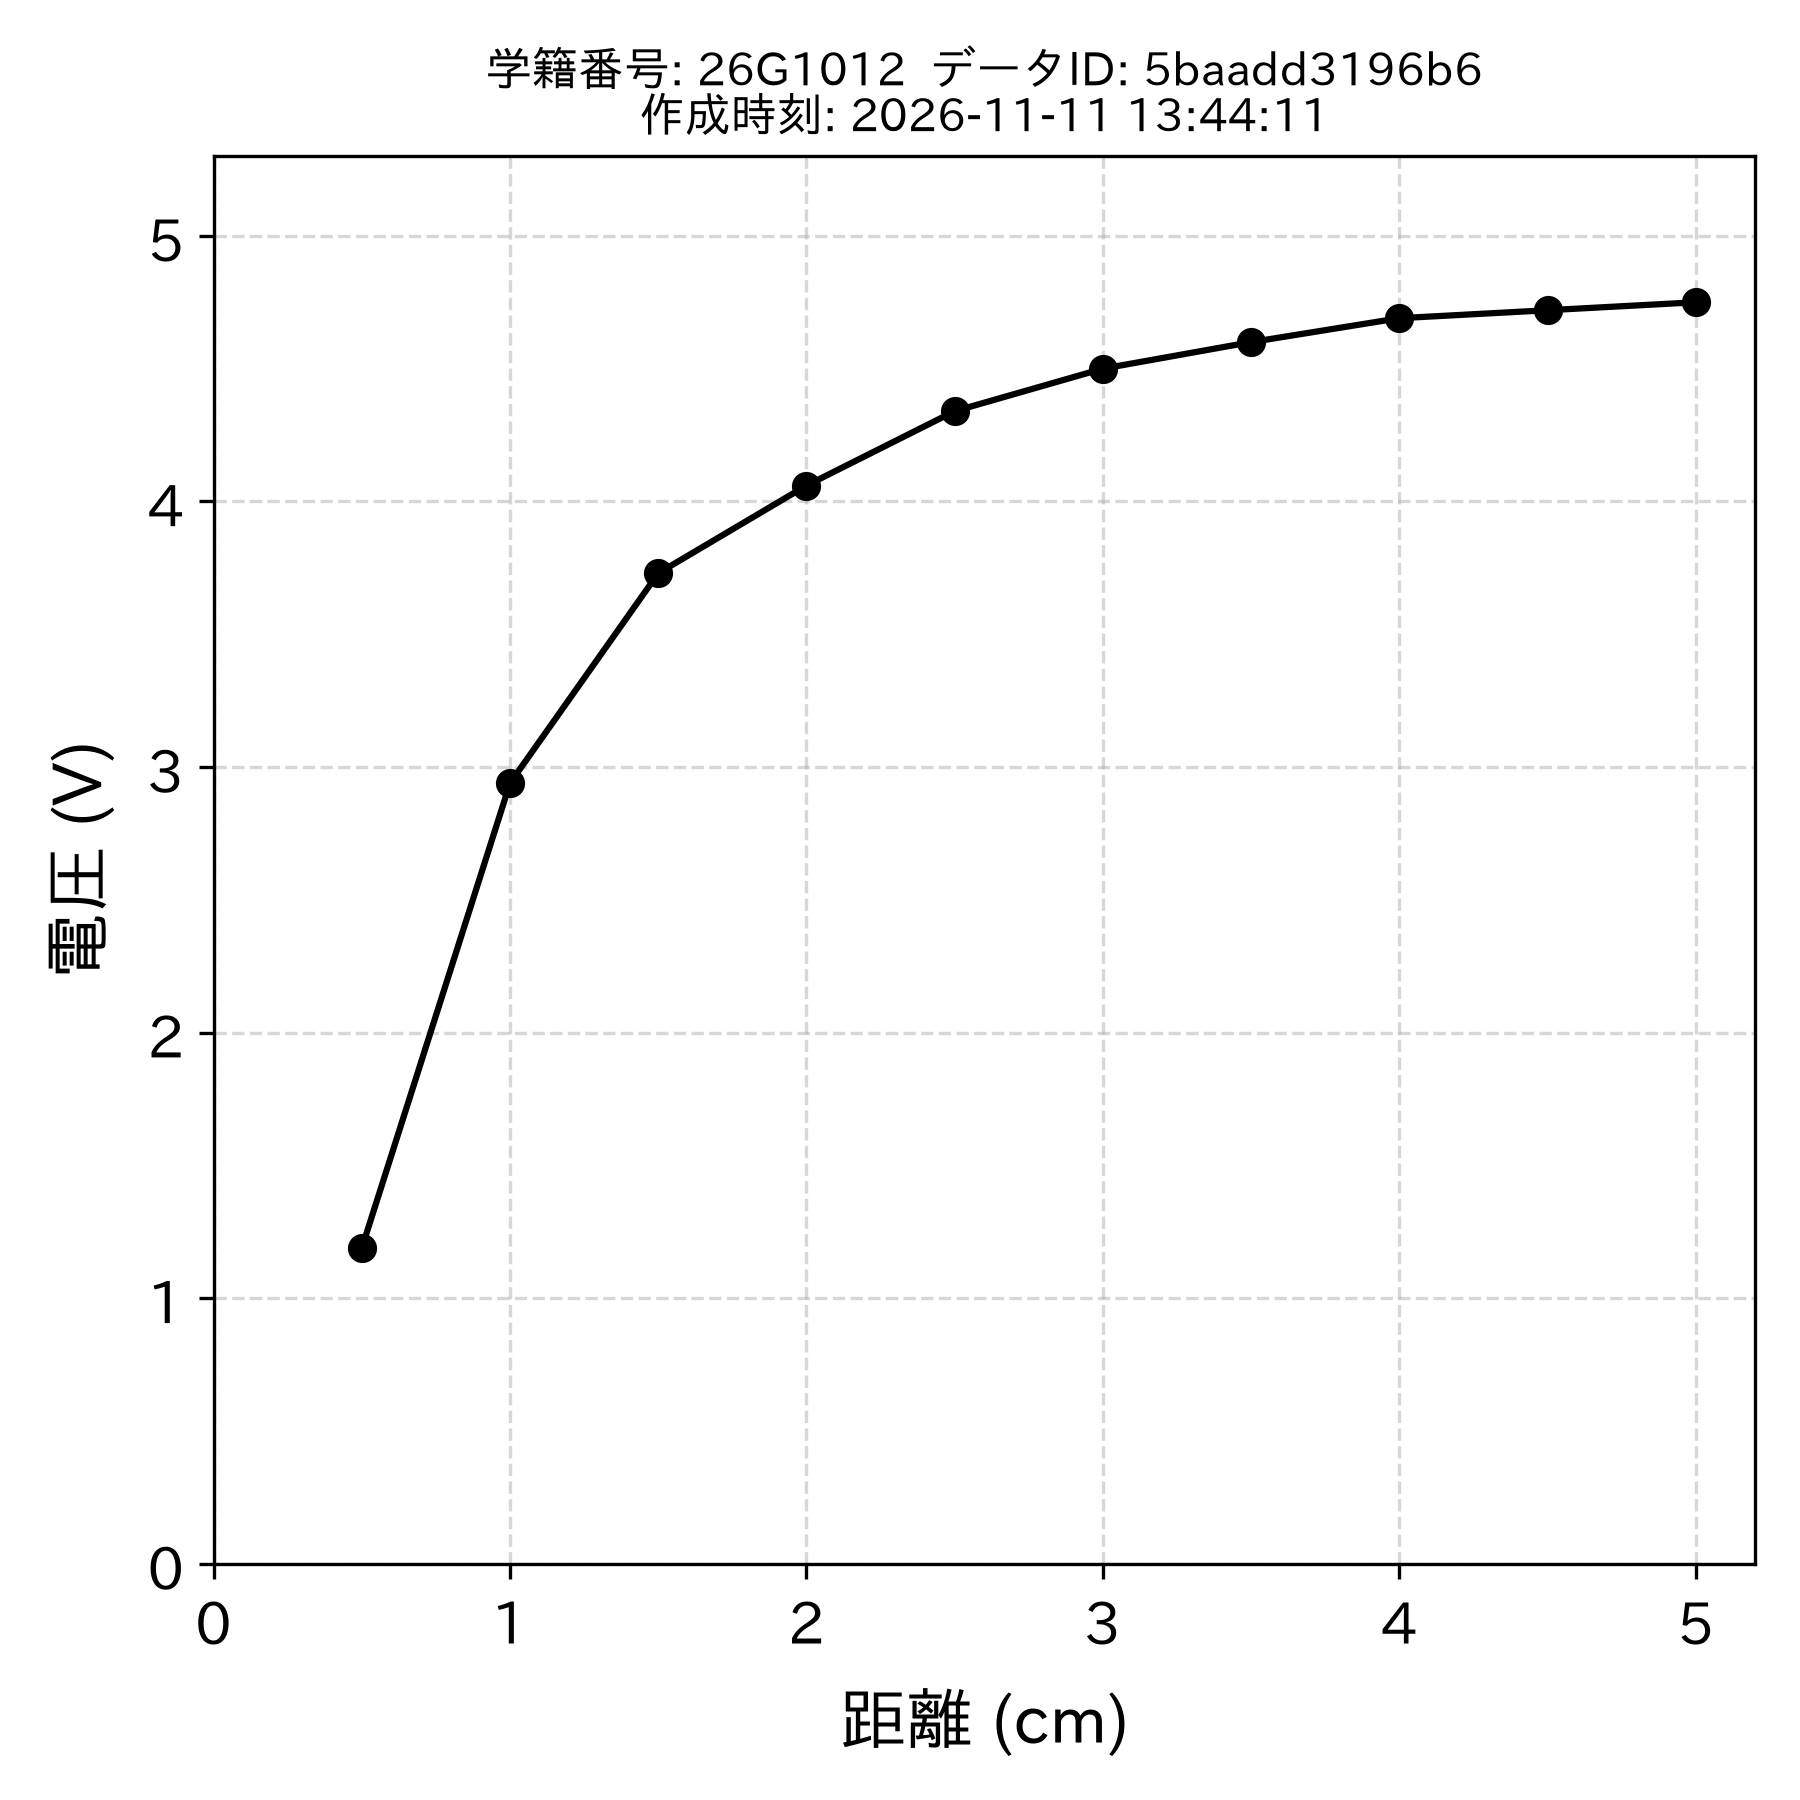
\includegraphics[width=0.65\textwidth,clip]{fig_work_C/result_C1.png}
  \caption{遮蔽物距離 $d$ に対する出力電圧 $V$ の測定結果（ワークC-1）}
  \label{fig:result_C1}
\end{figure}

図\ref{fig:result_C1}および表\ref{tab:c1_distance_voltage}より，遮蔽物距離 $d$ の増大に伴って測定電圧 $V$ は $1.19\,\mathrm{V}$ から $4.75\,\mathrm{V}$ へと単調に増加した．
特に，距離が $0.5\,\mathrm{cm}$ から $2.0\,\mathrm{cm}$ までの近距離領域では傾きが急峻であり，距離の増加に伴い電圧が急激に上昇した．
一方で，距離が $2.5\,\mathrm{cm}$ を超える遠距離領域では電圧変化率が徐々に低下し，電源電圧5\,Vに近い $4.7\,\mathrm{V}$ 付近で緩やかに飽和する非線形な応答特性が確認された．
また，測定電圧値はArduinoのLEDマトリクス上にリアルタイムで「1.19」「2.94」のように小数点付きで正しく表示されることを目視確認した．


\subsection{ワークC-2：CdSセルによる照度変化データの取得結果}

Arduinoをアクセスポイント（SSID: \texttt{ZZAP012}）として起動し，Pythonプログラムから $1.0\,\mathrm{s}$ 周期で100秒間にわたり取得したCdSセンサ回路の出力電圧波形を図\ref{fig:result_C2}に示す．

\begin{figure}[htbp]
  \centering
  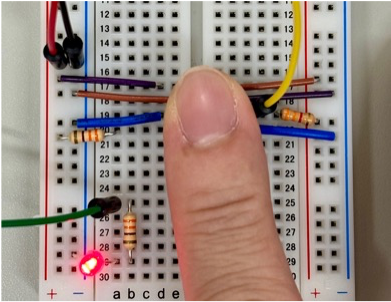
\includegraphics[width=0.85\textwidth,clip]{fig_work_C/result_C2.png}
  \caption{手の接近・離脱に伴うCdSセンサ回路の出力電圧波形（ワークC-2）}
  \label{fig:result_C2}
\end{figure}

図\ref{fig:result_C2}に示す通り，各測定フェーズにおける電圧挙動は以下の明確な段階的変化を示した：
\begin{enumerate}
    \item \textbf{0〜19\,s（非遮蔽定常状態）}：センサ上部が完全に開放された状態であり，室内照明光を直接受光して電圧は平均 $2.85\,\mathrm{V}$（$2.80 \sim 2.89\,\mathrm{V}$）で極めて安定に推移した．
    \item \textbf{20〜40\,s（上部約9\,cm遮蔽）}：手を9\,cm上空にかざした直後に電圧が平均 $3.36\,\mathrm{V}$（$3.16 \sim 3.40\,\mathrm{V}$）へとステップ状に上昇した．手の微小な揺れを反映して微小な変動が観測された．
    \item \textbf{41〜60\,s（上部約6\,cm遮蔽）}：手を6\,cmまで降下させると，受光面の影が濃くなり，電圧はさらに平均 $3.63\,\mathrm{V}$（$3.48 \sim 3.69\,\mathrm{V}$）まで一段高く跳ね上がり，その水準を維持した．
    \item \textbf{61〜80\,s（上部約3\,cm遮蔽）}：手を3\,cmまで近接させると，受光面が大きく覆われ，出力電圧は本実験中の最高値となる平均 $3.91\,\mathrm{V}$（最大 $3.94\,\mathrm{V}$）に達した．
    \item \textbf{81〜100\,s（遮蔽解除・復帰）}：手を瞬時に取り除くと，電圧は速やかに初期の基底水準（約 $2.80 \sim 2.98\,\mathrm{V}$）へと急落し，定常状態に復帰した．
\end{enumerate}
全101回の通信要求においてタイムアウトやパケットドロップは1件も発生せず，通信成功率 $100\%$ で連続データ記録が達成された．


\subsection{ワークC-3：時系列データの平滑化比較結果}

ワークC-2で取得した生波形（\texttt{voltage}）に対し，ウインドウサイズ $M=5$ の移動平均（\texttt{voltage\_MA}）および指数移動平均（\texttt{voltage\_EMA}）を適用した比較結果を図\ref{fig:result_C3}に示す．

\begin{figure}[htbp]
  \centering
  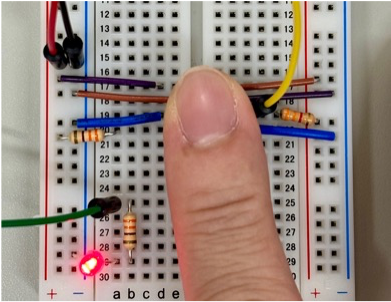
\includegraphics[width=0.85\textwidth,clip]{fig_work_C/result_C3.png}
  \caption{平滑化処理による波形比較（上：生データ，中：移動平均 MA，下：指数移動平均 EMA）}
  \label{fig:result_C3}
\end{figure}

図\ref{fig:result_C3}より，各平滑化処理の特徴は以下の通り確認された：
\begin{itemize}
    \item \textbf{生データ（上段）}：各定常区間において高周波の微小リップル（幅約 $0.05\,\mathrm{V}$）が頻繁に観測され，波形輪郭が粗い状態であった．
    \item \textbf{移動平均 MA（中段）}：定常領域の微小ノイズが均一に平滑化され，滑らかなトレースが得られた．しかし，手が接近・離脱した各ステップ境界（$t=20, 41, 61, 81\,\mathrm{s}$）において，立ち上がりおよび立ち下がりが5サンプル（5秒間）にわたって斜めに傾斜し，過渡変化に対する時間的遅れ（位相ラグ）が顕著に生じた．
    \item \textbf{指数移動平均 EMA（下段）}：MAと同様に定常部のノイズを十分に抑制しつつ，ステップ変化の立ち上がり初期においてMAよりも急峻に追従した．段差開始直後の1〜2サンプルで変化幅の過半を捉えており，過渡応答の応答遅延がMAに比べて大幅に軽減されている様子が確認された．
\end{itemize}


%-----------------------------------------------------------------------------------
\clearpage
\section{考察}

\subsection{フォトリフレクタにおける遮蔽物距離と出力電圧の物理的関係}
ワークC-1において，フォトリフレクタ（LBR-127HLD）と遮蔽物の距離 $d$ が増大するに伴い，出力電圧 $V_{\mathrm{out}}$ が単調増加し，遠距離で飽和する特性が得られた．この物理的要因について回路論および光学的知見に基づいて考察する．

フォトリフレクタは，赤外発光ダイオード（LED）からの放射光が遮蔽物表面で乱反射し，近接配置されたフォトトランジスタの受光面に入射することで動作する\cite{LBR-127HLD, 中村力1987ゲート蓄積型, wilson1998optoelectronics}．
点光源から出射された光の放射照度 $E$ は，幾何光学的な逆二乗則に従い\cite{iwasaki_point_method}，遮蔽物までの距離 $d$ の二乗に反比例して減衰する：
\begin{equation}
    E(d) \propto \frac{1}{d^2}
\end{equation}
さらに，遮蔽物表面で反射された光が再び距離 $d$ を伝搬してフォトトランジスタに入射するため，総合的な受光光束 $\Phi_r$ は近似的に距離の4乗に反比例，または素子間の幾何学的視野制限を考慮すると $d^{-2} \sim d^{-3}$ に比例して急激に低下する．

フォトトランジスタに光が入射すると，受光部半導体PN接合近傍で電子・正孔対が光電生成され，光電流 $I_p$ が発生する．これがトランジスタの直流電流増幅率 $h_{FE}$ によって増幅され，コレクタ電流 $I_C$ として流れる：
\begin{equation}
    I_C \approx h_{FE} \cdot I_p \propto \Phi_r(d)
\end{equation}
本測定回路では，電源電圧 $V_{CC} = 5\,\mathrm{V}$ とコレクタ端子の間にプルアップ抵抗 $R_L = 3.3\,\mathrm{k}\Omega$ を挿入しているため，出力電圧 $V_{\mathrm{out}}$ は，
\begin{equation}
    V_{\mathrm{out}} = V_{CC} - R_L \cdot I_C
    \label{eq:vout_pr}
\end{equation}
で決定される．
遮蔽物が至近距離（$d = 0.5\,\mathrm{cm}$）にある場合，受光光束 $\Phi_r$ が最大となり大きなコレクタ電流 $I_C$ が流れるため，抵抗 $R_L$ における電圧降下 $R_L I_C$ が約 $3.81\,\mathrm{V}$（$5.0 - 1.19 = 3.81\,\mathrm{V}$）に達し，出力電圧は $V_{\mathrm{out}} = 1.19\,\mathrm{V}$ と低くなる．
逆に，遮蔽物が遠ざかる（$d \ge 2.5\,\mathrm{cm}$）と，反射光束 $\Phi_r$ が著しく減少してフォトトランジスタは遮断状態（カットオフ， $I_C \to 0$）に漸近する．このため $R_L I_C \to 0$ となり，出力電圧は電源電圧 $5\,\mathrm{V}$ に極めて近い $4.75\,\mathrm{V}$ へと漸近・飽和する．
以上の解析より，実験で観測された非線形な単調増加曲線は，空間的光伝搬の減衰則と半導体プルアップ検出回路の動作原理に完全に整合していると結論付けられる．


\subsection{CdSセルの光電導効果と遮蔽距離に伴う抵抗変化の要因}
ワークC-2において，手をセンサ上空から段階的に接近させた際，出力電圧が $2.85\,\mathrm{V} \to 3.36\,\mathrm{V} \to 3.63\,\mathrm{V} \to 3.91\,\mathrm{V}$ と段階的に上昇した要因について，半導体の光電導効果および分圧回路の観点から考察する．

CdS（硫化カドミウム）はII-VI族化合物半導体であり，その禁制帯幅（バンドギャップエネルギー）は約 $2.42\,\mathrm{eV}$（波長換算で約 $515\,\mathrm{nm}$）である\cite{川口慎一朗1966cds, 石川太郎1974照明制御システムへの半導体応用}．
可視光（天井蛍光灯やLED照明の光）がCdS素子の受光面に入射すると，光子エネルギー $h\nu$ がバンドギャップを上回り，価電子帯の電子が伝導帯へ励起され，電子・正孔対が生成される．
励起されたキャリア密度 $\Delta n$ は入射光強度（照度 $L\,\mathrm{[lx]}$）に依存し，導電率 $\sigma = e(n\mu_n + p\mu_p)$ が増大するため，素子の内部抵抗 $R_{\mathrm{CdS}}$ は照度 $L$ に対して，
\begin{equation}
    R_{\mathrm{CdS}} \approx R_0 \cdot L^{-\gamma} \quad (\gamma \approx 0.7 \sim 0.9)
    \label{eq:cds_resistance_law}
\end{equation}
の関係に従って指数関数的に減少する\cite{石川太郎1974照明制御システムへの半導体応用}．

本回路では，5\,V電源側に固定抵抗 $R_F = 3.3\,\mathrm{k}\Omega$，GND側にCdSセルを接続した分圧回路を構成した．
したがって，A0端子における出力電圧 $V_{\mathrm{out}}$ は式(\ref{eq:cds_divider_actual})より，
\begin{equation}
    V_{\mathrm{out}} = 5.0 \times \frac{R_{\mathrm{CdS}}}{3.3\,\mathrm{k}\Omega + R_{\mathrm{CdS}}}
\end{equation}
となる．
\begin{enumerate}
    \item \textbf{遮蔽なし（開放定常時）}：受光面に直接照明光が入射するため $R_{\mathrm{CdS}}$ は約 $4.4\,\mathrm{k}\Omega$ となり，出力電圧は $V_{\mathrm{out}} = 5.0 \times \frac{4.4}{3.3 + 4.4} \approx 2.86\,\mathrm{V}$（実測平均 $2.85\,\mathrm{V}$）となる．
    \item \textbf{手の接近（9\,cm $\to$ 6\,cm $\to$ 3\,cm）}：手が接近するにつれて受光面に対する立体角的な光線遮蔽率が増大し，素子近傍の照度 $L$ が急激に低下する．式(\ref{eq:cds_resistance_law})に基づき，CdS内部のキャリア生成率が低下して再結合が支配的となり，暗抵抗化が進む．
    実測値より式(\ref{eq:cds_divider_actual})を逆算して得られた各高さにおけるCdS素子抵抗値 $R_{\mathrm{CdS}} = \frac{3.3 \times V_{\mathrm{out}}}{5.0 - V_{\mathrm{out}}}$ は，9\,cm時で約 $6.8\,\mathrm{k}\Omega$（$V_{\mathrm{out}} = 3.36\,\mathrm{V}$），6\,cm時で約 $8.7\,\mathrm{k}\Omega$（$V_{\mathrm{out}} = 3.63\,\mathrm{V}$），3\,cm時で約 $11.8\,\mathrm{k}\Omega$（$V_{\mathrm{out}} = 3.91\,\mathrm{V}$）へと単調に増大した．
\end{enumerate}
このように，受光面の照度低下がCdS素子のキャリア密度低下を招き，素子抵抗の増大を通じて分圧電位の上昇をもたらしたことが定量的・物理的に証明された．


\subsection{移動平均（MA）と指数移動平均（EMA）の平滑化特性の比較考察}
ワークC-3において，生信号に重畳するノイズの除去と過渡変化に対する追従性の観点から，移動平均（MA）と指数移動平均（EMA）を比較検討した結果について考察する．

\subsubsection{周波数応答とノイズ低減効果の理論比較}
サンプリング周期を $T_s = 1.0\,\mathrm{s}$（サンプリング周波数 $f_s = 1.0\,\mathrm{Hz}$）とする．
単純移動平均フィルタ（式(\ref{eq:ma_def})）の離散時間伝達関数 $H_{\mathrm{MA}}(z)$ は，
\begin{equation}
    H_{\mathrm{MA}}(z) = \frac{1}{M} \sum_{k=0}^{M-1} z^{-k} = \frac{1 - z^{-M}}{M(1 - z^{-1})}
\end{equation}
で与えられ，その振幅二乗特性（周波数伝達関数）はディリクレ核状のシンク関数型となり，
\begin{equation}
    |H_{\mathrm{MA}}(e^{j\omega})| = \frac{1}{M} \left| \frac{\sin(M\omega / 2)}{\sin(\omega / 2)} \right| \quad (\omega = 2\pi f / f_s)
\end{equation}
となる．周波数 $f = k \cdot f_s / M = k \cdot 0.2\,\mathrm{Hz}$（$k = 1, 2, \dots$）において完全にゼロ点（ノッチ）を持ち，周期的な変動成分を強力に遮断する．

一方，指数移動平均フィルタ（式(\ref{eq:ema_def})）の伝達関数 $H_{\mathrm{EMA}}(z)$ は1次の低域通過型IIRフィルタであり，
\begin{equation}
    H_{\mathrm{EMA}}(z) = \frac{\alpha}{1 - (1 - \alpha)z^{-1}}
\end{equation}
振幅特性は，
\begin{equation}
    |H_{\mathrm{EMA}}(e^{j\omega})| = \frac{\alpha}{\sqrt{1 + (1 - \alpha)^2 - 2(1 - \alpha)\cos\omega}}
\end{equation}
となる．$\alpha = 1/3$ のとき，直流（$\omega=0$）利得は1であり，高周波側（$\omega = \pi$）に向かって滑らかに減衰する．
このため，定常ノイズの分散低減率は，
\begin{equation}
    \sigma^2_{\mathrm{MA}} = \frac{1}{M} \sigma^2_{\mathrm{raw}} = 0.20 \cdot \sigma^2_{\mathrm{raw}}
\end{equation}
\begin{equation}
    \sigma^2_{\mathrm{EMA}} = \frac{\alpha}{2 - \alpha} \sigma^2_{\mathrm{raw}} = \frac{1/3}{2 - 1/3} \sigma^2_{\mathrm{raw}} = 0.20 \cdot \sigma^2_{\mathrm{raw}}
\end{equation}
となり，理論上の白色雑音に対する分散削減比率は両者ともに $20\%$（$1/5$）と完全に同一となる．実測波形の定常区間において，両者がほぼ同等水準の平滑度を示したことはこの理論結果と一致している．

\subsubsection{ステップ応答と応答遅延（位相遅れ）の比較}
両者の決定的な差異は，急激な照度変化（ステップ状変化）に対する過渡応答に現れた．
\begin{itemize}
    \item \textbf{MAの遅延特性}：MAは線形位相特性を持ち，その群遅延 $\tau_g$ はウインドウ全体の中央，すなわち，
    \begin{equation}
        \tau_g = \frac{M - 1}{2} = \frac{5 - 1}{2} = 2.0\,\mathrm{サンプル} \quad (2.0\,\mathrm{s})
    \end{equation}
    で一定である．ステップ変化が入力された際，5サンプル分のデータが完全に新しい値で満たされるまで均等な傾きで直線的に遷移するため，変化直後の立ち上がりが鈍重となり，急激なエッジの検出には不利となる．
    \item \textbf{EMAの追従特性}：EMAは過去のサンプルを指数関数的に忘却するが，現時刻のサンプルには最大の重み $\alpha = 0.333$ を直接反映する．ステップ変化直後の1サンプル目で最終変化量の約 $33.3\%$，2サンプル目で約 $55.6\%$，3サンプル目で約 $70.4\%$ まで急速に接近する．
    このため，図\ref{fig:result_C3}で確認されたように，段差の初期エッジをシャープに追従し，実時間での状態変化を検知する用途（閾値判定など）においてMAよりも優れた即応性を発揮する．
\end{itemize}
以上の考察より，オフライン解析や定常値の精密評価には厳密にゼロ点遮断を持つ移動平均（MA）が適し，リアルタイムモニタリングや状態遷移検出には初期応答遅延の小さい指数移動平均（EMA）が優位であるという実用的な選定基準が得られた．


%-----------------------------------------------------------------------------------
\section{おわりに}
本実習（ワークC）では，Arduino UNO R4 WiFiを用いて，LEDマトリクスによる自律的表示，Wi-Fi SoftAPを用いた組み込みWebサーバの構築，フォトリフレクタおよびCdSセルによるアナログ計測，ならびにPythonによる時系列データの収集と平滑化アルゴリズムの実装・評価を一貫して遂行した．

ワークC-1では，8×12 LEDマトリクス上に3桁の電圧値と小数点を正確に描画する制御プログラムを開発し，フォトリフレクタと遮蔽物間の距離特性を測定した．距離の逆二乗則に伴う反射光束の急激な減衰がプルアップ抵抗を介して出力電圧の単調増加および飽和傾向をもたらす物理メカニズムを実証した．
ワークC-2では，ESP32-S3による独自のWi-FiアクセスポイントとHTTP/JSONサーバを確立し，CdS光導電セルの受光照度変化に応じた電圧遷移を100秒間にわたり欠損なく取得することに成功した．
ワークC-3では，移動平均（MA）および指数移動平均（EMA）の平滑化フィルタを実装し，理論的ノイズ低減率が同等（$20\%$）である一方，EMAがステップ応答において優れた立ち上がり追従性を示し，過渡遅延の低減に有利であることを実証した．

これらの成果は，最終的な結合課題において，ワークAで設計した脈波検出回路のアナログ信号をワークBのアルゴリズムでピーク検出し，その測定結果（心拍数・脈波波形）をLEDマトリクスに即時表示するとともにWi-Fi経由で外部計算機へリアルタイム配信する，完全なワイヤレス生体モニタリングシステムの構築へと直結する重要な基盤技術となる．


%-----------------------------------------------------------------------------------
\clearpage
\section{付録：作成プログラム}

\subsection{ワークC-1で作成したプログラム}

\begin{lstlisting}[caption={ワークC-1 メインスケッチ (myprm.ino)}, label={lst:c1_myprm}]
#include "myLEDMatrix.h"

int analogValue = 0;
double measuredVoltage = 0.0;

void setup() {
  initLEDMatrix();
}

void loop() {
  analogValue = analogRead(A0);
  measuredVoltage = (double)analogValue / 1023.0 * 5.0;
  updateDisplayC1(measuredVoltage);
  delay(100);
}
\end{lstlisting}

\begin{lstlisting}[caption={ワークC-1 LED制御ヘッダ (myLEDMatrix.h)}, label={lst:c1_myledmatrix_h}]
#ifndef MyLEDMatrix_h
#define MyLEDMatrix_h
#include <Arduino.h>
#include "Arduino_LED_Matrix.h"

void initLEDMatrix();
void displayDigit(int d, int s_r, int s_c);
void updateDisplay(int v);
void updateDisplayC1(double v);
#endif
\end{lstlisting}

\begin{lstlisting}[caption={ワークC-1 LED制御実装 (myLEDMatrix.cpp)}, label={lst:c1_myledmatrix_cpp}]
#include "myLEDMatrix.h"

ArduinoLEDMatrix matrix;
int c, r;

byte frame[8][12] = {
    {0, 0, 0, 0, 0, 0, 0, 0, 0, 0, 0, 0},
    {0, 0, 0, 0, 0, 0, 0, 0, 0, 0, 0, 0},
    {0, 0, 0, 0, 0, 0, 0, 0, 0, 0, 0, 0},
    {0, 0, 0, 0, 0, 0, 0, 0, 0, 0, 0, 0},
    {0, 0, 0, 0, 0, 0, 0, 0, 0, 0, 0, 0},
    {0, 0, 0, 0, 0, 0, 0, 0, 0, 0, 0, 0},
    {0, 0, 0, 0, 0, 0, 0, 0, 0, 0, 0, 0},
    {0, 0, 0, 0, 0, 0, 0, 0, 0, 0, 0, 0}};

byte digits[5][30]{
    {1, 1, 1, 0, 0, 1, 1, 1, 1, 1, 1, 1, 1, 0, 1,
     1, 1, 1, 1, 1, 1, 1, 1, 1, 1, 1, 1, 1, 1, 1},
    {1, 0, 1, 0, 0, 1, 0, 0, 1, 0, 0, 1, 1, 0, 1,
     1, 0, 0, 1, 0, 0, 0, 0, 1, 1, 0, 1, 1, 0, 1},
    {1, 0, 1, 0, 0, 1, 1, 1, 1, 1, 1, 1, 1, 1, 1,
     1, 1, 1, 1, 1, 1, 0, 0, 1, 1, 1, 1, 1, 1, 1},
    {1, 0, 1, 0, 0, 1, 1, 0, 0, 0, 0, 1, 0, 0, 1,
     0, 0, 1, 1, 0, 1, 0, 0, 1, 1, 0, 1, 0, 0, 1},
    {1, 1, 1, 0, 0, 1, 1, 1, 1, 1, 1, 1, 0, 0, 1,
     1, 1, 1, 1, 1, 1, 0, 0, 1, 1, 1, 1, 1, 1, 1},
};

void initLEDMatrix() {
  matrix.begin();
}

void displayDigit(int d, int s_r, int s_c) {
  for (int r = 0; r < 5; r++) {
    for (int c = 0; c < 3; c++) {
      frame[s_r + r][s_c + c] = digits[r][d * 3 + c];
    }
  }
  matrix.renderBitmap(frame, 8, 12);
}

void updateDisplay(int v) {
  displayDigit(v % 10, 2, 9);
  displayDigit((v / 10) % 10, 2, 5);
  displayDigit((v / 100) % 10, 2, 1);
}

void displayDigitC1(int d, int s_r, int s_c) {
  for (int r = 0; r < 5; r++) {
    for (int c = 0; c < 3; c++) {
      frame[s_r + r][s_c + c] = digits[r][d * 3 + c];
    }
  }
  frame[7][4] = 1;  // 小数点の表示
  matrix.renderBitmap(frame, 8, 12);
}

void updateDisplayC1(double v) {
  displayDigitC1(int(v * 100) % 10, 2, 9);
  displayDigitC1((int(v * 100) / 10) % 10, 2, 5);
  displayDigitC1((int(v * 100) / 100) % 10, 2, 1);
}
\end{lstlisting}

\begin{lstlisting}[caption={ワークC-1 グラフ描画スクリプト (Python)}, label={lst:c1_plot}]
import matplotlib.pyplot as plt

d = [0.50, 1.00, 1.50, 2.00, 2.50, 3.00, 3.50, 4.00, 4.50, 5.00]
v = [1.19, 2.94, 3.73, 4.06, 4.34, 4.50, 4.60, 4.69, 4.72, 4.75]

plt.figure(figsize=(6, 6))
plt.plot(d, v, "ko-", markersize=6, linewidth=1.5)
plt.xlabel("距離 (cm)", fontsize=16, labelpad=8)
plt.ylabel("電圧 (V)", fontsize=16, labelpad=8)
plt.xlim(0, 5.2)
plt.ylim(0, 5.3)
plt.tick_params(labelsize=14)
plt.grid(True, linestyle="--", alpha=0.5)
plt.tight_layout()
plt.savefig("result_C1.png", dpi=300)
plt.show()
\end{lstlisting}


\subsection{ワークC-2で作成したプログラム}

\begin{lstlisting}[caption={ワークC-2 通信設定ヘッダ (config.h)}, label={lst:c2_config}]
#ifndef Config_h
#define Config_h

#define SECRET_SSID "ZZAP012"
#define SECRET_PASS ""
#define STUDENT_ID 12

#endif
\end{lstlisting}

\begin{lstlisting}[caption={ワークC-2 Webサーバヘッダ (myServer.h)}, label={lst:c2_myserver_h}]
#ifndef MyServer_h
#define MyServer_h

#include "WiFiS3.h"
#include "config.h"

void initServer();
void handleClientRequest(double sensorValue);

#endif
\end{lstlisting}

\begin{lstlisting}[caption={ワークC-2 Webサーバ実装 (myServer.cpp)}, label={lst:c2_myserver_cpp}]
#include "myServer.h"

char ssid[] = SECRET_SSID;
char pass[] = SECRET_PASS;
WiFiServer server(80);

void initServer() {
  WiFi.config(IPAddress(192, 168, STUDENT_ID, 2));
  if (WiFi.beginAP(ssid, pass) != WL_AP_LISTENING) {
    Serial.println("Failed to start access point");
    while (true);
  }
  server.begin();
  Serial.println("Server started");
}

void handleClientRequest(double sensorValue) {
  WiFiClient client = server.available();
  if (client) {
    String body = "{\"value\": " + String(sensorValue, 2) + "}";
    String currentLine = "";
    unsigned long startTime = millis();

    while (client.connected() && millis() - startTime < 1000) {
      if (client.available()) {
        char c = client.read();
        Serial.write(c);
        if (c == '\n') {
          if (currentLine.length() == 0) {
            client.println("HTTP/1.1 200 OK");
            client.println("Content-Type: application/json");
            client.println("Content-Length: " + String(body.length()));
            client.println("Connection: close");
            client.println();
            client.print(body);
            client.flush();
            break;
          } else {
            currentLine = "";
          }
        } else if (c != '\r') {
          currentLine += c;
        }
      }
    }
    client.stop();
  }
}
\end{lstlisting}

\begin{lstlisting}[caption={ワークC-2 データ取得スクリプト (Python)}, label={lst:c2_fetch}]
import requests, time, threading
import pandas as pd
import numpy as np

student_id = 12
url = f"http://192.168.{student_id}.2"
num_samples = 101
sample_interval = 1.0
recorded_data = []
latest_val = 0.0
http_session = requests.Session()

def fetch_worker():
    global latest_val
    try:
        res = http_session.get(url, timeout=sample_interval * 0.8)
        res.raise_for_status()
        latest_val = float(res.json()["value"])
    except Exception:
        pass

base_time = time.perf_counter()
for idx in range(num_samples):
    threading.Thread(target=fetch_worker, daemon=True).start()
    time.sleep(max(0, base_time + (idx + 1) * sample_interval - time.perf_counter()))
    recorded_data.append(latest_val)

pd.DataFrame({"voltage": recorded_data}).to_csv("result_C2.csv", index=False)
\end{lstlisting}


\subsection{ワークC-3で作成したプログラム}

\begin{lstlisting}[caption={ワークC-3 平滑化および比較描画スクリプト (Python)}, label={lst:c3_smooth}]
import pandas as pd
import numpy as np
import matplotlib.pyplot as plt

df = pd.read_csv("result_C2.csv")
v_raw = df["voltage"]
v_ma = v_raw.rolling(window=5).mean()
v_ema = v_raw.ewm(span=5, adjust=False).mean()

fig, (ax1, ax2, ax3) = plt.subplots(3, 1, figsize=(8, 8), sharex=True)
t_axis = np.arange(len(v_raw))

ax1.plot(t_axis, v_raw, "ko-", markersize=3, linewidth=1, label="voltage")
ax1.set_ylabel("電圧 (V)", fontsize=14)
ax1.set_ylim(2.0, 4.5)
ax1.grid(True, linestyle="--", alpha=0.5)
ax1.legend(loc="upper right", fontsize=12)

ax2.plot(t_axis, v_ma, "ro-", markersize=3, linewidth=1, label="voltage_MA")
ax2.set_ylabel("電圧 (V)", fontsize=14)
ax2.set_ylim(2.0, 4.5)
ax2.grid(True, linestyle="--", alpha=0.5)
ax2.legend(loc="upper right", fontsize=12)

ax3.plot(t_axis, v_ema, "bo-", markersize=3, linewidth=1, label="voltage_EMA")
ax3.set_xlabel("時間 (s)", fontsize=14, labelpad=8)
ax3.set_ylabel("電圧 (V)", fontsize=14)
ax3.set_ylim(2.0, 4.5)
ax3.set_xlim(0, 100)
ax3.grid(True, linestyle="--", alpha=0.5)
ax3.legend(loc="upper right", fontsize=12)

plt.tight_layout()
plt.savefig("result_C3.png", dpi=300)
plt.show()
\end{lstlisting}
